\section{Injections}
\label{sec:appendix_injections}

This chapter will show all options provided by injections. For a short introduction how to implement methods of the model, refer to chapter \ref{sec:intro_injections}.

In order to demonstrate injections we will provide functionality for saving our DoubleLinkedList to a file. Begin with an empty workspace, create a new metamodel ''Demo'' and replace the Demo.eap with the file from our .zip file. Now open Demo.eap and change the ''Default Language for Code Generation'' (Tools $\rightarrow$ Options $\rightarrow$ Source Code Engineering) to ''Ecore''. Add a method ''void toFile(EString path)'' to List (Fig. \ref{fig:append_inj_diagram}) and export the project to Eclipse.

\begin{figure}[htbp]
\begin{center}
  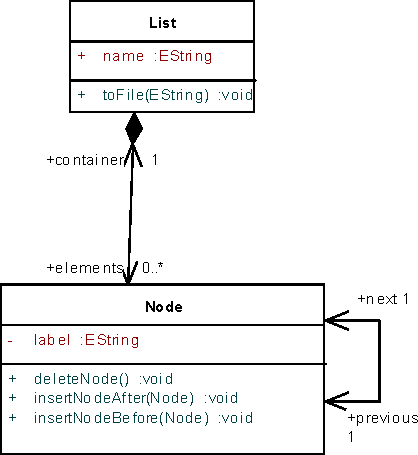
\includegraphics[width=0.4\textwidth]{pics/advancedTopics/injections/ea_diagram}
  \caption{Diagram of the DoubleLinkedList.}
  \label{fig:append_inj_diagram}
\end{center}
\end{figure}

To implement the ''toFile'' method, right-click gen/DoubleLinkedListLanguage/List.java in the generated project and choose ''eMoflon/create Injection for class'', which will generate the file injection/DoubleLinkedListLanguage/List.inject. Insert the code given in Fig. \ref{code:list_toFile_impl} to the file.

    \begin{figure}[htbp]
        \centering
        \begin{lstlisting}[language=Injection]
partial class List
{

    @model toFile(String path) <--

        try{

            FileWriter fstream = new FileWriter(path);
            BufferedWriter out = new BufferedWriter(fstream);
            out.write(this.toText());

            out.close();
        }catch (Exception e){
            System.err.println(e.toString);
        }

    -->

}
        \end{lstlisting}
        \caption{Implementation of List::toFile(String)}
        \label{code:list_toFile_impl}
    \end{figure}

To use the Eclipse template, type ''$@$'' and hit ''Ctrl+Shift'' and choose ''Inject method in model''. Functions that are annotated with ''\@ model'' implement methods that are defined in the interface of the model and habe the structure ''@model [signature] $<--$ [code] $-->$ ''.

You may have noticed that we use an undefined method ''List::toText()'' in the implementation of the ''toFile''. We will now implement this as a private method of List, but since List is only an Interface, we will add it only as a member to the implementation class: Right-click on gen/DoubleLinkedListLanguage/impl/ListImpl.java and choose again ''eMoflon/create Injection for class'', which will create you injection/DoubleLinkedListLanguage/impl/ListImpl.inject. Implement it with the code given in Fig. \ref{code:listImpl_toText_impl}.


\begin{figure}[htbp]
        \centering
        \begin{lstlisting}
import java.io.*;

partial class ListImpl
{
    @members <--

    private String toText(){
        StringBuilder sb = new StringBuilder();

        for(Node element : elements){
            sb.append(element.getLabel());
            sb.append("\n");
        }

        return sb.toString();
    }

    -->
}
        \end{lstlisting}
        \caption{Implementation of ListImpl.inject}
        \label{code:listImpl_toText_impl}
    \end{figure}

Note that we begin the implementation with the import of ''java.io.*''. This is necessary since the implementation of ''toFile'' will appear in ListImpl and will need this import. Member functions and fields are injected using the ''@members'' keyword. Everything in the surrounded area will be copied to the end of the ListImpl.java file, which enables you to add member functions and fields at will. You can even expand the interface of List this way, but this is a dirty way and should only be used for backward compatiblity. Note also that you can have several ''@model'' methods in you .inject file, but only one ''@member''.
The code will appear in ListImpl.java when you now rebuild the project (right-click on ''DoubleLinkedListLanguage'' and choose ''eMoflon/Build and clean'').